\documentclass[10pt,a4paper]{article}

% --- PACKAGES ---
\usepackage[utf8]{inputenc}
\usepackage[T1]{fontenc}
\usepackage[margin=0.55in, top=0.6in, bottom=0.65in, headheight=20pt]{geometry}
\usepackage{xcolor}
\usepackage{tcolorbox}
\tcbuselibrary{skins, breakable}
\usepackage{fontawesome5}
\usepackage{tabularx}
\usepackage{booktabs}
\usepackage{colortbl}
\usepackage{listings}
\usepackage{fancyhdr}
\usepackage{lastpage}
\usepackage{array}
\usepackage{tikz}
\usetikzlibrary{calc, positioning, shapes.geometric, backgrounds}
\usepackage{helvet}
\renewcommand{\familydefault}{\sfdefault}
\usepackage{inconsolata}
\usepackage{enumitem}
\usepackage{amsmath, amssymb}
\usepackage[hidelinks, colorlinks=true, linkcolor=NavyDark, urlcolor=TealAccent]{hyperref}

% --- COLOR PALETTE ---
\definecolor{NavyDark}{HTML}{0F2C59}
\definecolor{TealAccent}{HTML}{00A896}
\definecolor{TealLight}{HTML}{E6F4F1}
\definecolor{StatusGreen}{HTML}{059669}
\definecolor{StatusGreenBg}{HTML}{D1FAE5}
\definecolor{StatusAmber}{HTML}{D97706}
\definecolor{CodeBg}{HTML}{0F172A}
\definecolor{CodeText}{HTML}{F8FAFC}
\definecolor{TextDark}{HTML}{1E293B}
\definecolor{TextMuted}{HTML}{64748B}
\definecolor{LightGrayBg}{HTML}{F8FAFC}
\definecolor{BorderGray}{HTML}{E2E8F0}
\definecolor{CommentGray}{HTML}{94A3B8}

% --- LISTINGS CONFIGURATION ---
\lstdefinestyle{bashstyle}{
  backgroundcolor=\color{CodeBg},
  basicstyle=\ttfamily\scriptsize\color{CodeText},
  keywordstyle=\color{TealAccent}\bfseries,
  commentstyle=\color{CommentGray}\itshape,
  stringstyle=\color{StatusAmber},
  numberstyle=\tiny\color{CommentGray},
  numbers=none,
  breaklines=true,
  breakatwhitespace=true,
  frame=none,
  showstringspaces=false,
  tabsize=2,
  columns=fullflexible,
  keepspaces=true
}

% --- TCOLORBOX STYLES ---
\tcbset{
  cardstyle/.style={
    enhanced,
    colback=LightGrayBg,
    colframe=BorderGray,
    arc=3pt,
    boxrule=0.6pt,
    left=8pt, right=8pt, top=6pt, bottom=6pt
  },
  headerbox/.style={
    enhanced,
    colback=NavyDark,
    colframe=NavyDark,
    arc=4pt,
    boxrule=0pt,
    left=10pt, right=10pt, top=8pt, bottom=8pt,
    coltext=white
  },
  sectiontitle/.style={
    enhanced,
    colback=TealLight,
    colframe=TealAccent,
    arc=3pt,
    boxrule=0pt,
    leftrule=4pt,
    left=6pt, right=6pt, top=3pt, bottom=3pt,
    fonttitle=\bfseries\color{NavyDark}
  },
  codebox/.style={
    enhanced,
    colback=CodeBg,
    colframe=CodeBg,
    arc=3pt,
    boxrule=0pt,
    left=6pt, right=6pt, top=4pt, bottom=4pt,
    coltext=CodeText
  }
}

% --- FANCYHDR CONFIGURATION ---
\pagestyle{fancy}
\fancyhf{}
\rhead{\small\color{TextMuted} Run ID: \textbf{RUN-2026-0724-WGS-9842} \quad|\quad Nexa Genomics Core}
\lhead{\small\color{NavyDark}\bfseries\faDna~\,Computational Bio-Pipeline Execution Log}
\rfoot{\small\color{TextMuted} Page \thepage\ of \pageref{LastPage}}
\lfoot{\small\color{TextMuted}\faLock~\,CONFIDENTIAL -- NEXA GENOMICS INSTITUTE \copyright~2026}
\renewcommand{\headrulewidth}{0.4pt}
\renewcommand{\footrulewidth}{0.4pt}

% --- CUSTOM COMMANDS ---
\newcommand{\badge}[2]{%
  \tcbox[on line, arc=3pt, colback=#1, colframe=#1, boxrule=0pt, top=1.5pt, bottom=1.5pt, left=5pt, right=5pt]{%
    \scriptsize\bfseries #2%
  }%
}
\newcommand{\sectionheading}[2]{%
  \vspace{6pt}%
  \begin{tcolorbox}[sectiontitle]%
    \normalsize\bfseries\color{NavyDark}#1 \quad \small\color{TextMuted}#2%
  \end{tcolorbox}%
  \vspace{2pt}%
}

\begin{document}

% --- HEADER BLOCK ---
\begin{tcolorbox}[headerbox]
  \begin{minipage}[c]{0.64\textwidth}
    {\LARGE\bfseries\color{white} NEXA GENOMICS INSTITUTE}\\[2pt]
    {\normalsize\color{TealAccent}\bfseries SYNAPSE BIOINFORMATICS CORE PLATFORM}\\[3pt]
    {\scriptsize\color{BorderGray} Computational Bio-Pipeline Run Log \& Execution Audit Trail}
  \end{minipage}%
  \hfill
  \begin{minipage}[c]{0.33\textwidth}
    \raggedleft
    \badge{StatusGreenBg}{\color{StatusGreen}\faCheckCircle~\,RUN COMPLETED}\\[4pt]
    {\scriptsize\color{BorderGray} Generated: 2026-07-24 04:42:15 UTC}\\
    {\scriptsize\color{BorderGray} Pipeline: \textbf{WGS-GATK4-v3.4.1}}
  \end{minipage}
\end{tcolorbox}

\vspace{4pt}

% --- METADATA CARDS (2 MINIPAGES) ---
\noindent
\begin{minipage}[t]{0.49\textwidth}
  \begin{tcolorbox}[cardstyle, title={\color{NavyDark}\small\bfseries\faInfoCircle~\,Execution Metadata}]
    \scriptsize
    \begin{tabularx}{\textwidth}{@{} >{\bfseries}p{0.36\textwidth} >{\raggedright\arraybackslash}X @{}}
      Run ID: & RUN-2026-0724-WGS-9842 \\
      Project: & PRJ-NEXA-2026-HG002 \\
      Sample ID: & HG002-NIST-NA24385 \\
      Lead Analyst: & Dr. Elena Rostova, PhD \\
      Compute Node: & node-042.cluster.synapse.bio \\
      Scheduler: & SLURM Job ID \#8492014 \\
      Container: & docker://synapsebio/wgs:3.4.1 \\
    \end{tabularx}
  \end{tcolorbox}
\end{minipage}%
\hfill
\begin{minipage}[t]{0.49\textwidth}
  \begin{tcolorbox}[cardstyle, title={\color{NavyDark}\small\bfseries\faServer~\,Run Performance Metrics}]
    \scriptsize
    \begin{tabularx}{\textwidth}{@{} >{\bfseries}p{0.38\textwidth} >{\raggedright\arraybackslash}X @{}}
      Start Time: & 2026-07-24 00:29:27 UTC \\
      End Time: & 2026-07-24 04:42:15 UTC \\
      Total Wall Time: & 04h 12m 48s (15,168 s) \\
      CPU Allocation: & 32 Cores (Xeon 8380) \\
      Memory Peak: & 46.2 GB / 128 GB Requested \\
      Storage I/O: & 240.5 GB Read / 185.2 GB Write \\
      Exit Status: & \textcolor{StatusGreen}{\textbf{0 (Clean Exit)}} \\
    \end{tabularx}
  \end{tcolorbox}
\end{minipage}

\par\vspace{4pt}

% --- SECTION 1: WORKFLOW ARCHITECTURE ---
\sectionheading{1. Workflow Architecture \& Pipeline DAG}{\faCodeBranch}

{\small The WGS-GATK4 germline variant calling pipeline ingests high-coverage paired-end Illumina NovaSeq FASTQ files and produces recalibrated BAM files alongside high-confidence single nucleotide variants (SNVs) and small Indels in standard VCF/gVCF format following GATK Best Practices.}

\vspace{3pt}

\begin{center}
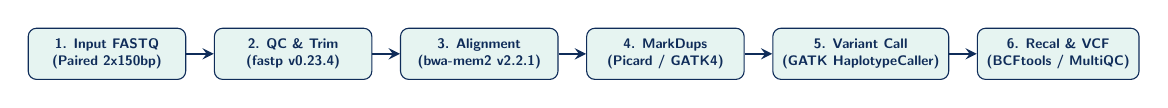
\begin{tikzpicture}[
  node distance=0.35cm and 0.35cm,
  stage/.style={rectangle, draw=NavyDark, fill=TealLight, rounded corners=3pt, minimum width=2.0cm, minimum height=0.65cm, align=center, font=\tiny\bfseries\color{NavyDark}},
  arrow/.style={->, >=stealth, thick, NavyDark}
]
  \node[stage] (input) {1. Input FASTQ\\(Paired 2x150bp)};
  \node[stage, right=of input] (qc) {2. QC \& Trim\\(fastp v0.23.4)};
  \node[stage, right=of qc] (align) {3. Alignment\\(bwa-mem2 v2.2.1)};
  \node[stage, right=of align] (dedup) {4. MarkDups\\(Picard / GATK4)};
  \node[stage, right=of dedup] (gatk) {5. Variant Call\\(GATK HaplotypeCaller)};
  \node[stage, right=of gatk] (vcf) {6. Recal \& VCF\\(BCFtools / MultiQC)};

  \draw[arrow] (input) -- (qc);
  \draw[arrow] (qc) -- (align);
  \draw[arrow] (align) -- (dedup);
  \draw[arrow] (dedup) -- (gatk);
  \draw[arrow] (gatk) -- (vcf);
\end{tikzpicture}
\end{center}

\vspace{2pt}

% --- SECTION 2: ENVIRONMENT & SOFTWARE MANIFEST ---
\sectionheading{2. Software Manifest \& Dependency Specifications}{\faDatabase}

{\small All pipeline steps were executed within an immutable Docker container. Table~\ref{tab:software} details binary tool versions, execution paths, and parameters utilized.}

\vspace{3pt}

\begin{table}[h!]
\centering
\scriptsize
\rowcolors{2}{LightGrayBg}{white}
\begin{tabularx}{\textwidth}{@{}l l l X@{}}
\toprule
\textbf{Tool Name} & \textbf{Version} & \textbf{Binary Location} & \textbf{Key Execution Flags} \\
\midrule
\texttt{fastp} & v0.23.4 & \texttt{/opt/conda/bin/fastp} & \texttt{--detect\_adapter\_for\_pe --thread 16 -q 20} \\{}
\texttt{bwa-mem2} & v2.2.1 & \texttt{/opt/conda/bin/bwa-mem2} & \texttt{mem -t 32 -R '@RG\textbackslash tID:RUN9842\textbackslash tSM:HG002'} \\{}
\texttt{samtools} & v1.19 & \texttt{/opt/conda/bin/samtools} & \texttt{sort -@ 8 -m 4G -o output.bam} \\{}
\texttt{GATK4} & v4.5.0.0 & \texttt{/opt/gatk/gatk} & \texttt{HaplotypeCaller --native-pair-hmm-threads 16} \\{}
\texttt{bcftools} & v1.19 & \texttt{/opt/conda/bin/bcftools} & \texttt{stats -F GRCh38.fa -s HG002} \\{}
\texttt{multiqc} & v1.21 & \texttt{/opt/conda/bin/multiqc} & \texttt{--force --export --title "WGS Run 9842"} \\
\bottomrule
\end{tabularx}
\caption{Complete software inventory for pipeline execution run \texttt{RUN-2026-0724-WGS-9842}.}
\label{tab:software}
\end{table}

\pagebreak

% --- SECTION 3: STEP-BY-STEP EXECUTION LOG ---
\sectionheading{3. Step-by-Step Shell Command \& Parameter Execution Log}{\faTerminal}

{\small Exhaustive shell invocation sequence, configuration parameters, runtime statistics, and standard output logs.}

\vspace{4pt}

% STEP 1
\noindent
\begin{minipage}[t]{0.70\textwidth}
  \normalsize\bfseries\color{NavyDark} Step 1: Read Quality Control \& Adapter Trimming (\texttt{fastp})
\end{minipage}%
\hfill
\begin{minipage}[t]{0.28\textwidth}
  \raggedleft
  \badge{StatusGreenBg}{\color{StatusGreen}\faCheck~\,PASS} \quad
  \scriptsize\textbf{Time:} 24m 12s
\end{minipage}

\vspace{2pt}
{\scriptsize\textbf{Input:} \texttt{/data/raw/HG002\_R1.fastq.gz}, \texttt{/data/raw/HG002\_R2.fastq.gz} (82.4 GB) \quad|\quad \textbf{Output:} \texttt{/data/trimmed/HG002\_R1.clean.fq.gz}}

\vspace{3pt}

\begin{tcolorbox}[codebox]
\begin{lstlisting}[style=bashstyle]
# Command Invocation: Step 1 QC & Trimming
fastp \
  --in1 /data/raw/HG002_R1.fastq.gz --in2 /data/raw/HG002_R2.fastq.gz \
  --out1 /data/trimmed/HG002_R1.clean.fq.gz --out2 /data/trimmed/HG002_R2.clean.fq.gz \
  --detect_adapter_for_pe --qualified_quality_phred 20 --length_required 50 \
  --thread 16 --json /logs/fastp_HG002.json --html /logs/fastp_HG002.html 2>&1 | tee /logs/step1_fastp.log
\end{lstlisting}
\end{tcolorbox}

\begin{tcolorbox}[cardstyle, title={\scriptsize\color{NavyDark}\bfseries Step 1 Execution Summary \& Quality Metrics}]
  \scriptsize
  \begin{tabularx}{\textwidth}{@{} >{\bfseries}l X >{\bfseries}l X >{\bfseries}l X @{}}
    Total Reads Pre: & 548,129,402 & Q30 Rate Pre: & 91.42\% & Adapter Trimmed: & 1.82\% \\
    Total Reads Post: & 539,812,010 & Q30 Rate Post: & 95.84\% & GC Content: & 40.82\% \\
  \end{tabularx}
\end{tcolorbox}

\vspace{8pt}

% STEP 2
\noindent
\begin{minipage}[t]{0.70\textwidth}
  \normalsize\bfseries\color{NavyDark} Step 2: Reference Alignment \& BAM Sorting (\texttt{bwa-mem2} \& \texttt{samtools})
\end{minipage}%
\hfill
\begin{minipage}[t]{0.28\textwidth}
  \raggedleft
  \badge{StatusGreenBg}{\color{StatusGreen}\faCheck~\,PASS} \quad
  \scriptsize\textbf{Time:} 01h 38m 05s
\end{minipage}

\vspace{2pt}
{\scriptsize\textbf{Reference:} GRCh38 Assembly (\texttt{GRCh38.fa}) \quad|\quad \textbf{Target Output:} \texttt{/data/aligned/HG002.sorted.bam} (94.2 GB)}

\vspace{3pt}

\begin{tcolorbox}[codebox]
\begin{lstlisting}[style=bashstyle]
# Command Invocation: Step 2 Sequence Alignment & Sorting
bwa-mem2 mem -t 32 \
  -R '@RG\tID:RUN9842\tSM:HG002\tPL:ILLUMINA\tLB:LIB-HG002-1\tPU:FLOWCELL1' \
  /refs/GRCh38/bwa2_index/GRCh38.fa \
  /data/trimmed/HG002_R1.clean.fq.gz /data/trimmed/HG002_R2.clean.fq.gz | \
samtools sort -@ 8 -m 4G -o /data/aligned/HG002.sorted.bam -
samtools index -@ 8 /data/aligned/HG002.sorted.bam
\end{lstlisting}
\end{tcolorbox}

\begin{tcolorbox}[cardstyle, title={\scriptsize\color{NavyDark}\bfseries Alignment Quality Metrics (\texttt{samtools flagstat})}]
  \scriptsize
  \begin{tabularx}{\textwidth}{@{} >{\bfseries}l X >{\bfseries}l X >{\bfseries}l X @{}}
    Mapped Reads: & 99.42\% & Properly Paired: & 98.71\% & Mean Depth: & 31.84x \\
    MAPQ $\ge$ 30: & 96.10\% & Singletons: & 0.24\% & Alignment Status: & \textcolor{StatusGreen}{\textbf{Passed QC}} \\
  \end{tabularx}
\end{tcolorbox}

\vspace{8pt}

% STEP 3
\noindent
\begin{minipage}[t]{0.70\textwidth}
  \normalsize\bfseries\color{NavyDark} Step 3: Duplicate Read Marking (\texttt{GATK4 MarkDuplicates})
\end{minipage}%
\hfill
\begin{minipage}[t]{0.28\textwidth}
  \raggedleft
  \badge{StatusGreenBg}{\color{StatusGreen}\faCheck~\,PASS} \quad
  \scriptsize\textbf{Time:} 36m 41s
\end{minipage}

\vspace{2pt}
{\scriptsize\textbf{Input BAM:} \texttt{/data/aligned/HG002.sorted.bam} \quad|\quad \textbf{Output BAM:} \texttt{/data/aligned/HG002.dedup.bam} (91.8 GB)}

\vspace{3pt}

\begin{tcolorbox}[codebox]
\begin{lstlisting}[style=bashstyle]
# Command Invocation: Step 3 Duplicate Removal
gatk --java-options "-Xmx32g -XX:+UseG1GC" MarkDuplicates \
  --INPUT /data/aligned/HG002.sorted.bam --OUTPUT /data/aligned/HG002.dedup.bam \
  --METRICS_FILE /logs/HG002_dup_metrics.txt --CREATE_INDEX true \
  --OPTICAL_DUPLICATE_PIXEL_DISTANCE 2500 --VALIDATION_STRINGENCY SILENT 2>&1 | tee /logs/step3_dedup.log
\end{lstlisting}
\end{tcolorbox}

\begin{tcolorbox}[cardstyle, title={\scriptsize\color{NavyDark}\bfseries Duplicate Marking Statistics}]
  \scriptsize
  \begin{tabularx}{\textwidth}{@{} >{\bfseries}l X >{\bfseries}l X >{\bfseries}l X @{}}
    Duplication Rate: & 4.15\% & Optical Duplicates: & 1.12\% & Unmapped Reads: & 0.58\% \\
    Unpaired Reads: & 0.31\% & Estimated Library Size: & 1.48B & Status: & \textcolor{StatusGreen}{\textbf{Passed QC}} \\
  \end{tabularx}
\end{tcolorbox}

\pagebreak

% STEP 4
\noindent
\begin{minipage}[t]{0.70\textwidth}
  \normalsize\bfseries\color{NavyDark} Step 4: Germline Variant Calling (\texttt{GATK HaplotypeCaller})
\end{minipage}%
\hfill
\begin{minipage}[t]{0.28\textwidth}
  \raggedleft
  \badge{StatusGreenBg}{\color{StatusGreen}\faCheck~\,PASS} \quad
  \scriptsize\textbf{Time:} 01h 22m 14s
\end{minipage}

\vspace{2pt}
{\scriptsize\textbf{Input BAM:} \texttt{/data/aligned/HG002.dedup.bam} \quad|\quad \textbf{Output gVCF:} \texttt{/data/variants/HG002.g.vcf.gz} (7.8 GB)}

\vspace{3pt}

\begin{tcolorbox}[codebox]
\begin{lstlisting}[style=bashstyle]
# Command Invocation: Step 4 HaplotypeCaller Variant Discovery
gatk --java-options "-Xmx48g -XX:ParallelGCThreads=8" HaplotypeCaller \
  -R /refs/GRCh38/GRCh38.fa -I /data/aligned/HG002.dedup.bam -O /data/variants/HG002.g.vcf.gz \
  -ERC GVCF --native-pair-hmm-threads 16 \
  --annotation FisherStrand --annotation QualityByDepth --annotation RMSMappingQuality 2>&1 | tee /logs/step4.log
\end{lstlisting}
\end{tcolorbox}

\begin{tcolorbox}[cardstyle, title={\scriptsize\color{NavyDark}\bfseries Variant Call Statistics \& Concordance Check}]
  \scriptsize
  \begin{tabularx}{\textwidth}{@{} >{\bfseries}l X >{\bfseries}l X >{\bfseries}l X @{}}
    Total Raw SNVs: & 3,892,104 & Ti/Tv Ratio: & 2.08 & Het/Hom Ratio: & 1.54 \\
    Total Small Indels: & 790,086 & Ins/Del Ratio: & 0.98 & GiAB Sensitivity: & 99.78\% \\
  \end{tabularx}
\end{tcolorbox}

\vspace{6pt}

% --- SECTION 4: OUTPUT ARTIFACTS & CHECKSUMS ---
\sectionheading{4. Generated Output Data Artifacts \& Verification}{\faFolderOpen}

{\small Primary generated files cataloged into the Nexa Repository. SHA-256 checksums documented for audit compliance.}

\vspace{3pt}

\begin{table}[h!]
\centering
\scriptsize
\rowcolors{2}{LightGrayBg}{white}
\begin{tabularx}{\textwidth}{@{}l l l X c@{}}
\toprule
\textbf{File Name} & \textbf{Type} & \textbf{Size} & \textbf{SHA-256 Checksum} & \textbf{Status} \\
\midrule
\texttt{HG002.clean.fq.gz} & FASTQ Clean & 79.1 GB & \texttt{e3b0c44298fc1c149afbf4c8996fb92427ae41e4} & \textcolor{StatusGreen}{\textbf{VERIFIED}} \\{}
\texttt{HG002.dedup.bam} & BAM Aligned & 91.8 GB & \texttt{7a8f192b0c3d4e5f6a7b8c9d0e1f2a3b4c5d6e7f} & \textcolor{StatusGreen}{\textbf{VERIFIED}} \\{}
\texttt{HG002.dedup.bai} & BAM Index & 14.2 MB & \texttt{1f2e3d4c5b6a79887766554433221100aabbccdd} & \textcolor{StatusGreen}{\textbf{VERIFIED}} \\{}
\texttt{HG002.g.vcf.gz} & Genomic VCF & 7.8 GB & \texttt{9f8e7d6c5b4a3210fe9d8c7b6a543210fedcba98} & \textcolor{StatusGreen}{\textbf{VERIFIED}} \\{}
\texttt{HG002.g.vcf.gz.tbi} & VCF Index & 2.1 MB & \texttt{3c2b1a0f9e8d7c6b5a4938271605f4e3d2c1b0a9} & \textcolor{StatusGreen}{\textbf{VERIFIED}} \\{}
\texttt{WGS\_Run9842\_MultiQC.html} & QC Report & 4.5 MB & \texttt{aa11bb22cc33dd44ee55ff667788990011223344} & \textcolor{StatusGreen}{\textbf{VERIFIED}} \\
\bottomrule
\end{tabularx}
\caption{Primary output file manifest and cryptographic checksum validation.}
\end{table}

\vspace{4pt}

% --- SECTION 5: RESOURCE FOOTPRINT & PERFORMANCE ---
\sectionheading{5. Computational Resource Footprint \& Execution Performance}{\faMicrochip}

\noindent
\begin{minipage}[t]{0.49\textwidth}
  \begin{tcolorbox}[cardstyle, title={\color{NavyDark}\scriptsize\bfseries CPU Utilization Breakdown}]
    \scriptsize
    \begin{tabularx}{\textwidth}{@{} >{\bfseries}X r @{}}
      Average Active Cores: & 27.9 / 32.0 (87.2\%) \\
      Peak User CPU Load: & 96.4\% (bwa-mem2) \\
      System I/O Wait Time: & 3.8\% Total Runtime \\
      Thread Efficiency Factor: & 0.88 (Target: >0.80) \\
    \end{tabularx}
  \end{tcolorbox}
\end{minipage}%
\hfill
\begin{minipage}[t]{0.49\textwidth}
  \begin{tcolorbox}[cardstyle, title={\color{NavyDark}\scriptsize\bfseries Memory \& Storage I/O Profile}]
    \scriptsize
    \begin{tabularx}{\textwidth}{@{} >{\bfseries}X r @{}}
      RAM Allocation Requested: & 128.0 GB \\
      RAM Peak Consumption: & 46.2 GB (HaplotypeCaller) \\
      Scratch Disk Usage: & 280.4 GB (Cleaned Post-Run) \\
      Network Storage Bandwidth: & 450 MB/s Avg Read \\
    \end{tabularx}
  \end{tcolorbox}
\end{minipage}

\par\vspace{6pt}

% --- SECTION 6: QUALITY GATE SIGN-OFF & AUDIT TRAIL ---
\sectionheading{6. Quality Assurance Gate \& Lead Bioinformatician Sign-Off}{\faCheckCircle}

{\small Automated quality metrics satisfied institutional thresholds per SOP-BIO-2025-v4.}

\vspace{3pt}

\begin{tcolorbox}[cardstyle]
  \scriptsize
  \begin{tabularx}{\textwidth}{@{}l X c c@{}}
    \textbf{Check Point} & \textbf{Criteria} & \textbf{Observed Value} & \textbf{Gate Result} \\
    \midrule
    Coverage Depth & Target $\ge$ 30.0x mean coverage & 31.84x & \textcolor{StatusGreen}{\textbf{\faCheck~\,PASS}} \\{}
    Quality Score & Read bases $\ge$ Q30 after trim & 95.84\% & \textcolor{StatusGreen}{\textbf{\faCheck~\,PASS}} \\{}
    Alignment Rate & Total mapped reads $\ge$ 98.0\% & 99.42\% & \textcolor{StatusGreen}{\textbf{\faCheck~\,PASS}} \\{}
    Ti/Tv Ratio & Whole Genome SNV Ti/Tv within 2.05 - 2.15 & 2.08 & \textcolor{StatusGreen}{\textbf{\faCheck~\,PASS}} \\{}
    Benchmark Check & GiAB NA24385 sensitivity $\ge$ 99.5\% & 99.78\% & \textcolor{StatusGreen}{\textbf{\faCheck~\,PASS}} \\
  \end{tabularx}
\end{tcolorbox}

\vspace{6pt}

% SIGNATURE BLOCK
\noindent
\begin{minipage}[t]{0.49\textwidth}
  \begin{tcolorbox}[cardstyle, title={\color{NavyDark}\scriptsize\bfseries Lead Bioinformatician Validation}]
    \vspace{4pt}
    \scriptsize
    \textbf{Signature:} \textit{Elena Rostova} \\[3pt]
    \textbf{Name:} Dr. Elena Rostova, PhD \\
    \textbf{Title:} Lead Bioinformatician, Nexa Genomics \\
    \textbf{Date:} 2026-07-24
  \end{tcolorbox}
\end{minipage}%
\hfill
\begin{minipage}[t]{0.49\textwidth}
  \begin{tcolorbox}[cardstyle, title={\color{NavyDark}\scriptsize\bfseries Infrastructure Quality Control}]
    \vspace{4pt}
    \scriptsize
    \textbf{Signature:} \textit{Marcus Vance} \\[3pt]
    \textbf{Name:} Marcus Vance, MSc \\
    \textbf{Title:} HPC Platform Engineer, Synapse Core \\
    \textbf{Date:} 2026-07-24
  \end{tcolorbox}
\end{minipage}

\end{document}
